% This is samplepaper.tex, a sample chapter demonstrating the
% LLNCS macro package for Springer Computer Science proceedings;
% Version 2.20 of 2017/10/04
%
\documentclass[runningheads]{llncs}
%

\usepackage{array}
\newcolumntype{C}[1]{>{\centering\arraybackslash}p{#1}}

\usepackage{graphicx}
\usepackage{csquotes}
\usepackage{multirow}
\usepackage{tikz}
\def\checkmark{\tikz\fill[scale=0.4](0,.35) -- (.25,0) -- (1,.7) -- (.25,.15) -- cycle;}

% Used for displaying a sample figure. If possible, figure files should
% be included in EPS format.
%
% If you use the hyperref package, please uncomment the following line
% to display URLs in blue roman font according to Springer's eBook style:
% \renewcommand\UrlFont{\color{blue}\rmfamily}

\begin{document}
%
\title{Market Research on GANs in Finance}
%
%\titlerunning{Abbreviated paper title}
% If the paper title is too long for the running head, you can set
% an abbreviated paper title here
%
\author{Leonardo Mandruzzato}
%
\authorrunning{L. Mandruzzato}
% First names are abbreviated in the running head.
% If there are more than two authors, 'et al.' is used.
%
\institute{ISTIC, Université de Rennes 1, Beaulieu - Bâtiment 12D, \\263 Avenue du Général Leclerc, 35042 Rennes, France \\ \email{leonardo.mandruzzato@etudiant.univ-rennes1.fr}}
%
\maketitle              % typeset the header of the contribution
%
\begin{abstract}
This paper discusses Generative Adversarial Networks (GANs), mainly focusing on their application in Finance. I did not take care of the technician aspects of the technology, but instead, I conducted market research on it.

The paper will describe the technology (section \ref{intro}), also looking at it from a broader perspective (section \ref{wider}). Then, taking as example the financial time series modelling task, it will compare GANs with the most relevant models used to accomplish it — i.e.,  ARCH/GARCH and ABMs  — trying to figure out the technology delta (section \ref{delta}). This document will also analyze the barriers for an entity that tries to enter the market with a business model that involves this technology (section \ref{GTM}). Moreover, I will describe a possible future scenario in which GANs are state-of-the-art and the business role that might develop due to their increasing usage (section \ref{future}). Finally, I will consider the current adoption of this network in the industry and how it can dramatically change in the years (section \ref{adoption}).

\keywords{ GANs \and ARCH/GARCH \and ABMs }
\end{abstract}
%
%
%
\section{Introduction}\label{intro}
With the word “GANs”, we refer to a series of machine learning frameworks introduced by Ian Goodfellow and his collaborators in 2014 \cite{goodfellow_2014}. 
They gained attention due to the effectiveness they have in image generation.  This technology is already very used in computer vision. Even though there are already several applications in finance \cite{eckerli_2021}, these frameworks are still considered novelties compared to other fields.

“Generative”, in the name “Generative Adversarial Network”, refers to a class of statistical models that contrasts with discriminative models. Given a set of data $X$ and a set of labels $Y$, a discriminative model captures the conditional probability $P(Y|X)$. On the other side, a generative model captures the joint probability $P(X, Y)$, or just $P(X)$ if there are no labels \cite{jebara_2004}. However, the original GAN framework does not foresee an exclusive use of generative models but exploits an adversarial process to obtain the final result. Thus, there are two different models (usually neural networks) involved in the training process. There is a generative model, the Generator ($G$), that captures the data distribution and generates new data starting from an input noise $Z$. Then, there is a classifier, the Discriminator ($D$), which estimates the probability that a sample comes from the training data and not from $G$. The Generator is responsible for the generation of data, and the Discriminator has the task of assessing the quality of the generated data providing feedback to the Generator.

Generally, the final aim is to discover patterns in the input data and learn them in a way that the model can then generate new samples that retain characteristics of the original dataset.

\begin{figure}
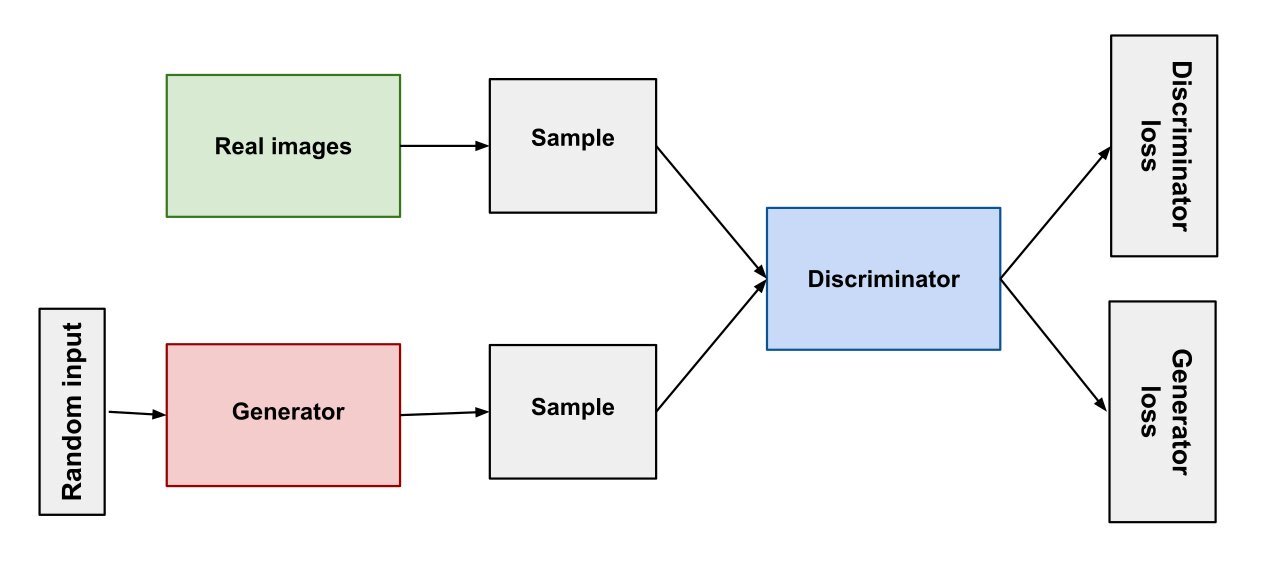
\includegraphics[width=\textwidth]{gan_diagram.jpg}
\caption{Original proposed GANs architecture}
\end{figure}

\section{Wider Perspective}\label{wider}
To make a broader analysis of the impact that this technology can have, we can frame it in a specific business model to forecast the possible consequences. Let’s imagine being in the shoes of a financial institution that is adopting this new tool. As we can read in \cite{dilmegani_2021}:

\begin{displayquote}
Financial institutions can leverage synthetic data, or data that is generated artificially based on real data, to overcome privacy (and other) challenges and provide innovative products and services to their customers.

[...]

Synthetic data can eliminate the risks of sharing. Instead of the original dataset, financial institutions can share synthetic data that preserves the important characteristics of the original dataset.
\end{displayquote}

From this quotation and also going through Assefa et al. \cite{AMEX}, we can extract three main aims to pursue for financial institutions:

\begin{itemize}
  \item overcoming privacy issues with synthetic data. In some ways, we can use synthetic data instead of anonymizing real ones (“Internal data use restrictions”, “Data sharing” in \cite{AMEX})
  \item obtain more inputs for training other models whether there is a lack of training data (“Tackling class imbalance”, “Training advanced Machine Learning models” in \cite{AMEX})
  \item create data representing new conditions on which test other models — i.e., stress test (“Lack of historical data” in \cite{AMEX})
\end{itemize}

These three key points may have interesting social and scientific repercussions.

\subsection{PESTL(E) Analysis}

\subsubsection{Political.}\label{political}
The politic could incentivize to use this technology to meet very marked social needs such as privacy and data protection issues, especially when it comes to banking data.
\subsubsection{Economic.}
Economically speaking, there might be several benefits in using this technology, and all of them are related to the improvement of the already existing AI models. Through GANs, we would be able to create synthetic data for those situations in which we have a small quantity of information — e.g., a crisis. It means that the financial institution would improve its models in use, especially when it comes to unlikely situations that are usually very delicate to manage.
\subsubsection{Social.}
As already mentioned in the paragraph \ref{political}, information privacy and data protection are social issues that have been quite felt in the last decade. GANs can only help in finding a solution for this complex problem.
\subsubsection{Technology.}
Even though we are only at the beginning of the development process of GANs for finance, and the math behind these models is very complex, there are already excellent results. However, researchers will refine GANs in the next five years as they did in the computer vision industry. In fact, in the last seven years, we have seen a stunning improvement in this technology applied to the creation of synthetic images (see Pic. \ref{improvement}).

\begin{figure}
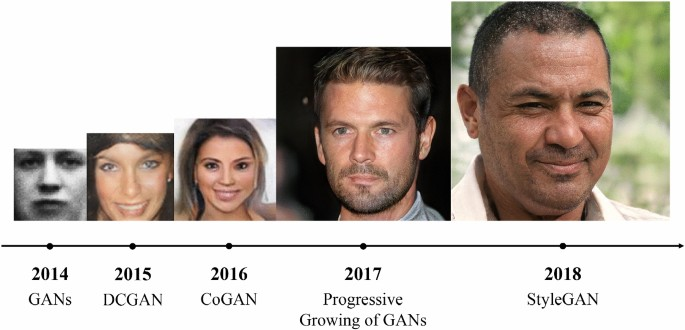
\includegraphics[width=\textwidth]{gan_improvement.jpg}
\caption{Image generation improvement from 2014 to 2018.}\label{improvement}
\end{figure}

\subsubsection{Legal.}
Usually, when we talk about AI in the legal sphere, there are several unresolved ethical topics. But, this is not the case, it is actually the opposite. Through synthetic data generation, we will be able to solve some issues related to privacy — e.g., sharing data between two different financial institutions or between two business lines within the same financial institution. It will lead the financial industry to an enormous step forward.

There is a final piece to consider when we analyze the legal sphere and GANs: explainability. We do not need a model able only to sample synthetic data that retains the features of real ones. We also need a clear explainability of the reason why we considered that output a good one. It is not relevant only to understand how the model produces specific data, but we also need to have a strong knowledge of the validation process that brought us to consider that data effective. Since the output of GANs will be the input of the following model, and the latter can then be questioned in the legal field, it is fundamental to have a solid explanation of why that data has been used to train or test that model.

\section{Technology Delta}\label{delta}
To make an analysis on how GANs actually perform we must follow a specific procedure. Firstly, we have to choose a task to accomplish (section \ref{task}). Secondly, we must find the features that characterize the original data we want to replicate (see section \ref{facts}). Then, we must select the technologies to compare GANs with (section \ref{models}). Finally, we analyze which technology better reproduces the selected characteristics in the output \ref{diff}. In this way, we would be able to conduct a qualitative analysis of the technology delta.

\subsection{Task to Accomplish}\label{task}
To perform this analysis, we are going to use as an example task the financial time-series modelling. To frame this task, we can quote Matignon 2007 \cite{matignon_2007}:

\begin{displayquote}
Time series models are widely used in economics, business and engineering to predict the seasonal variability of a target variable over time, where past values are used as the input variables for the model.
\end{displayquote}

\subsection{Stylized Facts}\label{facts}
The dynamics of financial markets are the perfect examples of complex phenomena. A big part of the underlying mechanics of the process is still unknown. However, lots of researches highlighted how the variations of asset prices share several significant statistical properties. The latter are known in the literature as stylized facts. We can mention here the ones we are going to use to make the comparison between different models, but there are others relevant too \cite{cont_2000}: 

\begin{itemize}
  \item absence of autocorrelation — i.e., linear unpredictability
  \item heavy tails — i.e., fat-tailed distribution
  \item gain-loss asymmetry
  \item volatility clustering
  \item leverage effect
\end{itemize}

\subsection{Previous Models} \label{models}
In literature, the two most known approaches to model financial time-series are stochastic processes \cite{engle_1982,bollerslev_1986} and agent-based models \cite{holland_1991}. 

Stochastic processes such as ARCH and GARCH describe a financial time-series as a series of random variables with temporally dependent parameters. However, it is hard to recover all the major stylized facts with such explicit mathematical formulations \cite{malmsten_2010}. 

In contrast, agent-based models (ABMs) describe agents’ behavior and interaction with other agents and the environment based on reasonable assumptions. However, it is difficult to design such agents’ behavior to calibrate a large number of model parameters based on real data. Moreover, making assumptions on the financial markets biases the final result because they are often wrong.

\subsection{Performances Differences}\label{diff}
Since the previous approaches still have issues, it is desirable to develop an alternative one with high reproducibility of stylized facts and built without apriori assumptions. Deep learning, especially deep generative models, provides such a solution.

Stochastic models — i.e., GARCH — can reproduce the absence of autocorrelation and the heavy-tailed distribution. Moreover, Given and Lins \cite{siven_2009} found a way to evolve the model (EGARCH) to reproduce also the leverage effect and the gain/loss asymmetry.

On the other side, ABMs mainly focus on reproducing heavy-tailed distribution and volatility clustering. Chen et al. \cite{chen_2013} designed a microscopic agent-based model able to also replicate leverage effects in addition to the stylized facts previously mentioned.

If we consider the FIN-GAN model \cite{fin_gan}, we can already observe, from a qualitative point of view, how GANs can reproduce a higher number of stylized facts (see table \ref{tab_fin_gan}). 

Moreover, if we do not only consider the stylized facts, but we also analyze some evaluation metrics to compare the distributions of synthetic and real data \cite{quant_gan}, we would notice how the previous approach (GARCH) is outperformed by GANs (see table \ref{tab_quant_gan}).

In conclusion, we can say that the technology delta between GANs and their predecessors is significant. This new technology can retain more statistical properties from the authentic data, being also more precise in doing so.

\begin{table}
\caption{Extract from a table of Takahashi et al. \cite{fin_gan}. Reproducibility of stylized facts with generators. N/A indicates that reproducibility is not reported. FIN-GAN is able to reproduce a higher number of stylized facts with respect to the previous methods.}\label{tab_fin_gan}
\begin{center}
    \begin{tabular}{ | C{1.6cm} | C{2.7cm} | C{2.1cm} | C{1.8cm} | C{1.5cm} | C{1.9cm} | }
    \hline
    \multirow{2}{3em}{\textbf{model}} &  \textbf{linear unpredictability} & \textbf{heavy-tailed distribution} & \textbf{volatility clustering} & \textbf{leverage effect} & \textbf{gain/loss asymmetry} \\
    \hline
    EGARCH \cite{siven_2009} & \multirow{2}{1em}{\checkmark} & \multirow{2}{1em}{\checkmark} & \multirow{2}{1em}{X} & \multirow{2}{1em}{\checkmark} & \multirow{2}{1em}{\checkmark}\\
    \hline
    Chen et al. \cite{chen_2013} & \multirow{2}{1em}{\checkmark} & \multirow{2}{1em}{\checkmark} & \multirow{2}{1em}{\checkmark} & \multirow{2}{1em}{\checkmark}& \multirow{2}{1em}{N/A}\\
    \hline
    FIN-GAN (MLP-CNN) \cite{fin_gan} & \multirow{3}{1em}{\checkmark} & \multirow{3}{1em}{\checkmark} & \multirow{3}{1em}{\checkmark} & \multirow{3}{1em}{\checkmark} & \multirow{3}{1em}{\checkmark} \\
    \hline
    \end{tabular}
\end{center}
\end{table}

\begin{table}
\caption{Extract from a table of Wiese et al. \cite{quant_gan}. Evaluated metrics for two out of three models applied — i.e., Quant GAN and GARCH. EMD = Earth Mover Distance \cite{EMD}. DY = Dragulescu and Yakovenko metric \cite{DY}. ACF = AutoCorrelation Function score. For each row, the best value is printed bold. The GARCH model is clearly outperformed by GANs. }\label{tab_quant_gan}
\begin{center}
    \begin{tabular}{ | C{2.3cm} | C{2.4cm} | C{2.3cm} | C{2.3cm} | }
    \hline
    & & \textbf{Quant GAN (TCN)} & \multirow{2}{6.5em}{\textbf{GARCH(1,1)}} \\
    \hline
    \multirow{8}{8em}{Distributional Metrics} & EMD(1) & \textbf{0.0039} & 0.0199 \\
    & EMD(5) & \textbf{0.0039} & 0.0145 \\
    & EMD(20) & \textbf{0.0040} & 0.0276 \\
    & EMD(100) & \textbf{0.0154} & 0.0935 \\
    & DY(1) & \textbf{19.1199} & 32.7090 \\
    & DY(5) & \textbf{21.1167} & 27.4760 \\
    & DY(20) & \textbf{26.3294} & 39.3796 \\
    & DY(100) & \textbf{28.1315} & 47.4779 \\
    \hline
    \multirow{4}{8em}{Dependence Scores} & ACF(id) & \textbf{0.0212} & 0.0223 \\
    & ACF($|\cdot|$) & \textbf{0.0248} & 0.0291 \\
    & ACF($(\cdot)^2$) & \textbf{0.0214} & 0.0253 \\
    & Leverage effect & \textbf{0.3291} & 0.4636 \\
    \hline
    \end{tabular}
\end{center}
\end{table}

\section{GTM Barriers}\label{GTM}
The barriers to enter a market usually depend on the business model in which we frame the technology. A financial institution will have different obstacles compared to a startup. 

However, we can individuate a common obstacle shared from different approaches: the implementation of an actual performing model that can recreate trusted data according to the criteria identified in the section \ref{facts}. As I mentioned multiple times, we are not at the state-of-the-art regarding this technology. Thus, we must wait until GANs reach a level of development that can allow us to start seriously operating with them.

For certain specific business models, input data can represent a huge barrier. We know that GANs need some initial data to learn the associated distribution. This data can be public — e.g., stock trend — or private — e.g., customer financial profiles.
For instance, a startup that wants to firstly design generative models and then sell them to financial institutions would encounter insurmountable difficulties in convincing the latter to share data to use as initial input due to privacy issues. 

Hence, only financial institutions can start spreading the usage of GANs when it comes to recreating private data. Fortunately, the AI labs of the major financial institutions in the world are already researching and experimenting with this technology (JP Morgan \cite{JP}, Financial Conduct Authority \cite{sandbox,FCA}, American Express \cite{AMEX}).

\section{GANs in the Future}\label{future}
\subsection{Possible Future Scenario}
There are different levels from which analyze a possible future scenario where GANs are in full use:

\begin{itemize}
  \item generative models will be able to solve most of the problems related to the invasion of information privacy
  \item financial business will change dramatically, and the words "cooperation" and "sharing" will no longer be taboo
  \item management of delicate and unlikely situations will be at least improved, and customer confidence in financial institutions will be greater
\end{itemize}

\subsubsection{Privacy.}
Generative models will create synthetic data able to maintain the same feature as the original ones. This affirmation is valid not only in finance but also in several other industries. With such technology, we will solve a big part of privacy and data protection issues. There will no longer be motivations for a company to illegally share private data when it can reach the same results legally. Privacy will no longer be a matter of ethical and moral decisions to take by companies’ directors, but it will only require the efficiency of security systems that will not allow attackers to steal data.

\subsubsection{Financial Business.}
Joint ventures between different financial institutions will become more frequent. From Assefa et al. \cite{AMEX}:

\begin{displayquote}
By sharing data between institutions and within the research community, better solutions can be found for technical problems faced by financial institutions. Sharing of synthetic data allows financial institutions to do this in a way that satisfies their data sharing restrictions. 
\end{displayquote}

A sort of cooperation between financial and non-financial entities — i.e., other companies, startups, research teams, universities — will be more manageable and a game-changer.

Furthermore, inside the same bank, the different business units will be more efficient working harmoniously together.

\subsubsection{Improved Models.}
Advanced machine learning models will benefit from the presence of more training and testing data. Especially for those models that actively work during certain events — e.g., flash crashes in the market, recessions, new regimes of behavior, the models, there will be an enormous improvement. Since the mentioned events are often delicate, having better technologies to face those critical happenings could help financial institutions increase their customers' confidence.

\subsection{Developing Business Roles}
In general, data experts — i.e., data engineers, data scientists, quant analysts, and machine learning engineers — are enough to model and develop GANs. However, due to the development of the technology, there is the possibility that a new business position originates in the years: the synthetic data quality assurance engineer. Mainly, its tasks would be to study and deeply understand how the authentic data are structured — e.g., for time series, the stylized facts — and then, conscious of the main features on which pay attention, evaluate the quality of the synthetic data produced by the generative models. Its role will be to support data engineers during the information retrieving, then the data scientists and machine learning engineers to model the networks, and finally the data / quantitative analysts to study and eventually validate the results obtained. Since GANs can recreate several types of data (numerical, categorical binary), there will be dozens of domains of specialization for engineers who want to pursue a career in this role.

\section{Diffusion}\label{adoption}
The GANs diffusion in the financial industry has already begun, but we are distant to reach the state-of-the-art. Currently, we have a Proof of Concept (PoC), but, in the future years, we will obtain extraordinary outcomes.

However, to let the usage of this technology to take off, it is essential to convince more entities to adopt this solution and not only a niche. For doing so, it would be necessary to cross the so-called chasm and pass from the early adopters to the early majority.

\subsection{Early Adopters}
As already mentioned in section \ref{GTM}, the early adopters must be the biggest players in the financial industry or, generalizing, entities with enormous availability of quality financial data (eventually also GAFAM \cite{GAFAM}). With the right amount of data, the subject can experiment and carry on high-quality researches on this technology. Unfortunately, they cannot share these data with external entities for obvious legal constraints, so they cannot make joint researches. There are not several entities with the availability of the resources — both human and economic — required to undertake this development path and bring GANs to a higher level. But, luckily, the biggest financial institutions in the industry are already working on it to keep up (JP Morgan \cite{JP}, Financial Conduct Authority \cite{sandbox,FCA}, American Express \cite{AMEX}).

\subsection{Crossing the Chasm}
Crossing the chasm and moving from the early adopters to the early majority is not easy at all. Today, carrying on high-level researches on GANs applied to financial data can be done by a niche. Inside the latter, there are all those players owning an enormous quantity of private and non-shareable data. Once these few actors find a solution to pass from PoCs to state-of-the-art models, they will recreate synthetic data so similar to the real ones that they will start sharing/selling it and practically passing it off as authentic. We can say that the final objective is to reach a situation where sharing synthetic data almost coincides with sharing original ones. The ability to share this data would enable other external and more modest actors to join the researches and further improve the state-of-the-art models obtained by the larger players. In the end, we would reach an extremely cooperative environment that would bring several benefits to the financial industry, not only for improving tools such as GANs but for all the shades of the business.

\section{Conclusions}
To sum up, I see in GANs an enormous potential to disrupt the financial industry. Furthermore, this technology will be the best solution to face and solve privacy and data protection issues. It will enable cooperation between different actors changing irreversibly the way to approach problems. It will unlock the possibility for financial institutions to outsource problems to specialized external actors able to find better solutions. Customer satisfaction will benefit a lot and, consequently, there will be greater confidence in the financial sector that will lead us to a more prosperous economy.
%
% ---- Bibliography ----
%
% BibTeX users should specify bibliography style 'splncs04'.
% References will then be sorted and formatted in the correct style.
%
% \bibliographystyle{splncs04}
% \bibliography{mybibliography}
%
\begin{thebibliography}{8}
\bibitem{goodfellow_2014}
Ian J. Goodfellow, Jean Pouget-Abadie, Mehdi Mirza, Bing Xu, David Warde-Farley, Sherjil Ozair, Aaron Courville, Yoshua Bengio. (2014). Generative Adversarial Networks.

\bibitem{eckerli_2021}
Florian Eckerli, Joerg Osterrieder. (2021). Generative Adversarial Network in Finance: an Overview.

\bibitem{jebara_2004}
Tony Jebara. (2004). Machine Learning. Discriminative and Generative.

\bibitem{dilmegani_2021}
Cem Dilmegani. (2021). 4 Synthetic data applications to enable finance innovation in ’21.
\url{https://research.aimultiple.com/synthetic-data-finance/}

\bibitem{AMEX}
Dmitry Efimov, Di Xu, Luyang Kong, Alexey Nefedov, Archana Anandakrishnan. (2020). Using Generative Adversarial Networks to Synthesize Artificial Financial Datasets.

\bibitem{matignon_2007}
Randall Matignon. (2007). Data Mining Using SAS Enterprise Miner.

\bibitem{cont_2000}
Rama Cont. (2000). Empirical properties of asset returns: stylized facts and statistical issues.

\bibitem{engle_1982}
Robert F. Engle. (1982). Autoregressive Conditional Heteroscedasticity with Estimates of the Variance of United Kingdom Inflation.

\bibitem{bollerslev_1986}
Tim Bollerslev. (1986). Generalized autoregressive conditional heteroskedasticity.

\bibitem{holland_1991}
John H. Holland, John H. Miller. (1991). Artificial Adaptive Agents in Economic Theory.

\bibitem{malmsten_2010}
H. Malmsten, T. Teräsvirta. (2010). Stylized facts of financial time series and three popular models of volatility.

\bibitem{siven_2009}
Johanne V. Siven, Jeffrey T. Lins. (2009). Gain/loss asymmetry in time series of individual stock prices and its relationship to the leverage effect.

\bibitem{chen_2013}
Jun-Jie Chen, Bo Zheng, L. Tan. (2013). Agent-based model with asymmetric trading and herding for complex financial systems.

\bibitem{fin_gan}
Shuntaro Takahashi, Yu Chen, Kumiko Tanaka-Ishii. (2019). Modeling financial time-series with generative adversarial networks.

\bibitem{quant_gan}
Magnus Wiese, Robert Knobloch, Ralf Korn, Peter Kretschmer. (2020). Quant GANs: Deep Generation of Financial Time Series.

\bibitem{EMD}
Cédric Villan. (2008). Optimal transport, old and new.

\bibitem{DY}
Adrian A. Dragulescu, Victor .M Yakovenko. (2002). Probability distribution of returns in the Heston model with stochastic volatility.

\bibitem{JP}
Samuel Assefa. (2020). Generating synthetic data in finance: opportunities, challenges and pitfalls.

\bibitem{FCA}
Financial Conduct Authority, City of London. (2021). Supporting innovation in financial services: the digital sandbox pilot.

\bibitem{sandbox}
Financial Conduct Authority, City of London. (2021). Digital Sandbox Pilot.
\url{https://www.digitalsandboxpilot.co.uk}

\bibitem{GAFAM}
Stephen Ajulu. (2020). Why Big Tech Firms Want A Piece Of Finance.
\url{https://medium.com/macoclock/why-big-tech-firms-want-a-piece-of-finance-deb375bcf1bb}

\end{thebibliography}
\end{document}
